
\documentclass[12pt]{article}

\usepackage{scicite}
\usepackage{times}
\usepackage{graphicx}
\usepackage{hyperref}
\usepackage{enumitem}
\usepackage{amsmath}
\usepackage[utf8]{inputenc}

\topmargin -1.5cm
\oddsidemargin 0.0cm
\textwidth 16cm 
\textheight 23.5cm
\footskip 1.0cm

\newenvironment{sciabstract}{%
\begin{quote} \bf}
{\end{quote}} 

\newcounter{lastnote}
\newenvironment{scilastnote}{%
  \setcounter{lastnote}{\value{enumiv}}%
  \addtocounter{lastnote}{+1}%
  \begin{list}%
  {\arabic{lastnote}.}
  {\setlength{\leftmargin}{.22in}}
  {\setlength{\labelsep}{.5em}}
}
{\end{list}}

\title{Assignment 3} 

\author
{Filipe Pires [85122], João Alegria [85048]\\
\\
Information Retrieval\\
\normalsize{Department of Electronics, Telecommunications and Informatics}\\
\normalsize{University of Aveiro}\\
} 

\date{\today{}}

%%%%%%%%%%%%%%%%% END OF PREAMBLE %%%%%%%%%%%%%%%%

\begin{document} 
\baselineskip18pt
\maketitle 

\section{Introduction}

This report was written for the discipline of 'Information Retrieval' and 
describes the implementation and evaluation of a ranked retrieval method that 
uses the indexes created with the solutions developed for the previous assignments.

We include the correction of design flaws of the delivery done prior to this one
and the updates applied both to the text corpus indexation and to our class diagram.
We also provide the instructions on how to run our code.

Along with the description of the solution, we also present the results of our
calculations to evaluate the solution and determine its efficiency according to 
the metrics proposed for this last assignment \cite{assign3}.
All code and documentation is present in our public GitHub project at 
\url{https://github.com/joao-alegria/RI}. 

\newpage
\section{Re-Indexing the Corpus}

In order to make query searches flexible, it was proposed to us the reindexation
of the text corpus considering not only the document titles but also their abstracts.
This turned out to be quite challenging due to its computational weight, as 
the abstracts were considerably larger than the titles.
The initial index occupied about 500Mb in disk, whereas the reindexation turned
out to be over 3Gb large.

There were 2 approaches when adding the abstract processing to our indexing process. 
The first one would consist in dealing with titles and abstracts separately,
creating independent index entries for both. 
This approach has the advantage of simplifying the process of verification of 
appearance of a given term in titles, abstracts or both, since they would be 
stored in different structures.
It has however the clear disadvantage of requiring far more disk space to store
all the information and introducing redundancy and unnecessary repetitions.

With this in mind, we went for another strategy, consisting of concatenating 
both fields and processing the resulting text as a whole.
This approach's advantage and disadvantage are inverted when compared to the 
previous, since the redundancy no longer exists but it becomes impossible to
distinguish the field a term appears at.
Our choice was based on the analysis of the requirements for the ranked retriever
we wanted to implement, as there seemed to be no need to keep the notion of where
each term appeared at in each document.
This also made the code adaptations to the indexing pipeline more straightforward 
and, as we previously mentioned, the final size in disk of the index smaller.
The execution time of this pipeline thankfully did not evolve as fast as the
disk space, passing from 20 minutes without the abstract to approximately 1 hour
and 20 minutes with it.

\newpage
\section{Ranked Retrieval of Relevant Documents}

With an entirely functional index creator and a folder of generated indexes from
the corpus of text documents, it was now time to develop a program capable of
interpreting queries and returning the index entries most relevant to them.
In this chapter we describe our implementation of a query results ranked retriever
- that we called \texttt{Searcher}.
We also explain how we prepared it for memory limitations and present the 
updates done to our class diagram.

\subsection{Document Ranked Scores}

The file \texttt{Searcher.py} contains an abstract class called \texttt{Searcher}
that serves as a template for the implementations of results retriever classes.
For our purposes, we developed \texttt{IndexSearcher}, a class that extends from
the abstract template and is capable of selecting which index files will be 
required to answer a given query, assigning scores to documents from the index
and returning the documents considered most relevant to the query according to 
these scores.

The step of determining which index files will be needed to answer the query
is done through the function \textit{retrieveRequiredFiles()} and is basically
a comparison of each query term of the query with the name of each index file. To obtain those tokens, logically the tokenizing process must be identical if not the same as the one used when indexing the entire corpus. Not doing so may compromise significantly the efficiency of the process.
As each index file is named after the first and last terms it contains (separated
by an underscore) and as the entire index is alphabetically ordered, the function
simply determines where each term will be present and returns those index files. A special case occurs when the necessary information is cached, i.e., the results are already present in memory. This memory management will be further detailed in the section \ref{memory}.

Calculating the score of each document regarding a query is not as easy to explain. The function \textit{calculateScores()} is the one responsible for obtaining the relevant document ids and the respective score values. With the the required files established and the indication if como information is already cached the score calculation may start. It's necessary to iterate over all the necessary files and identify the lines were the query tokens appear, so that we have access to the documents where that specific term occurred; as a execution time and memory reduction mechanism we implemented a champion list strategy to decrease our search space, meaning that we only consider the first N documents (N can be defined by the user), which is made easy by the fact that previously with our indexing process we already order the posting list (list of documents were a term appeared) by the tf-idf weight calculated on that process too.

Once knowing the champion list for each term we know which documents are relevant to that query, assuming that having at least one term of the query is enough. Of course, not all documents have the same relevance to the user, a document that have all the query terms may be more relevant that others with only one term. A score is then calculated to allow the ordering of the several documents following the formulas:

\begin{equation}
  \label{score}
  Score_{d} = \sum_{t=0}^{nT} W_{qt} * W_{dt}
\end{equation}

\begin{equation}
  \label{simple}
  W_{qt} = 1 + \log(tf) * idf => Simplifying => W_{qt} = 1 * idf
\end{equation}

Where \ref{score} shows that the score of a document is obtained by the sum of the multiplications of the query term weight by the weight of the term in the document. This formula although not too complex can be simplified, as shown by formula \ref{simple}. Since the execution time when retrieving information is crucial, the more simple and straightforward the process can be, the best it is for the user. The simplification that we implemented consist in assuming that each term occurs only once in the query, which that doesn't compromise the performance of the search, since the terms are still considered and the number of times a term appears in the query will not affect the relevance of a document. This allow our process to simply skip the step of calculating the query terms weight as shown by \ref{simple}, which can translate in crucial processing time.

Once the scores are found, \textit{sortAndWriteResults()} does what its name 
suggests: sorts the documents by score and writes to a results file the first K
documents, where K is passed as argument by the user.

\subsection{Relevance Feedback}

We knew \texttt{IndexSearcher} was a very limited solution, as it considers 
documents as relevant only for the presence of query terms in their titles 
and/or abstracts.
So the idea of attempting to expand queries was introduced through feeding back
to the Searcher information that would help it fine tune its results.

The aim of relevance feedback is to try to steer the search process behavior in a way that guides the results to more relevant document, this is accomplished by transforming the query vectors (consisting in the
weights of each query term in the query) into new vectors closer to the actually
relevant documents and further away from the remainder.
The way we implemented this form of attempting to improve results was through 
a well known algorithm named Rocchio algorithm.

Rocchio was developed using the Vector Space Model like many other relevance feedback approaches. Descending from the SMART Information Retrieval System, the algorithm assumes that most users have a general conception of which documents should be denoted as relevant or non-relevant. With this information in mind, a improvement over the classic score values calculation is proposed by following the formula:

\begin{equation}
  \vec{q}_{m} = \alpha\vec{q}_{0} + \beta\frac{1}{|D_{r}|} \sum_{ \vec{d}_{j} \in D_{r}} \vec{d}_{j} - \gamma\frac{1}{|D_{nr}|} \sum_{ \vec{d}_{j} \in D_{nr}} \vec{d}_{j}
\end{equation}

Where $\vec{q}_{0}$ is the original query vector, i.e., the weights of each term in the query, that in our context, with the simplification is $1*idf$, the $D_{r}$ is the list of known relevant documents and $D_{nr}$ is the list of known non-relevant documents; finally $\alpha, \beta, \gamma$ are parameters that can be fine tunned by the user to improve the performance of the algorithm. Developing a bit the formula we end up with the addition of three vectors, the original query, the sum of all relevant document vectors and the sum of all nun-relevant vectors, which when applying the formula and summing all the values of the resulting vector we achieve the new score of the document.

Taking a closer look on what the algorithm attempts to do, in a first analysis it appears to do the same for all documents, which could translate in maintaining the relations between then, but it's from our understanding that although thats true, referring to the vector space model that the algorithm has its base that what's really happening is that the algorithm is trying to shift the query closer to the relevant documents by the addition of its middle point ($\frac{1}{|D_{r}|} \sum_{ \vec{d}_{j} \in D_{r}} \vec{d}_{j}$) and distance it from the non-relevant documents through the substation of its middle point ($\frac{1}{|D_{nr}|} \sum_{ \vec{d}_{j} \in D_{nr}} \vec{d}_{j}$). This algorithm had a considerable impact in our system, which will be further explained in section \ref{results} and section \ref{discussion}.

We decided to implement 2 distinct approaches of providing feedback, i.e., the relevant and non-relevant documents to the algorithm. The first was a simulation of the user feedback and the other was a pseudo feedback. To achieve the first strategy we executed the information retrieval normally, obtaining the best results our system could supply and compared the obtained top K results with the gold standard supplied to us. From those, the results that checked with the gold standard were considered as relevant documents and the remaining as irrelevant; this information was partially processed and persisted in files to make its further usage easier. A similar process was made to the pseudo feedback, being this one quite simpler since it only considers the relevant documents and defines them by selecting the top K values returned.

A Python script was developed to perform all this automatically, and being an auxiliary function we didn't took in consideration the execution time nor the memory usage, since the values it produces should ideally, in a real world situation, be selected and verified in a more controlled and reliable way.

\subsection{Memory Management} \label{memory}
When developing our searcher we decided to implement an intelligent memory usage strategy to take advantage of the unused memory that the system has available. By storing the terms and the respective champions needed to answer the queries performed in the system, as well as the number of times the term is used, we can manage which terms and documents are in memory and which ones should we maintain, which theoretically should be the most important ones.

The workflow that we adopted consisted in if the program has memory available it will store the terms used to answer the query being processed and the respective champion lists. If the system detects that the memory limit is close to be surpassed, the internal cache is cleaned, leaving only one forth of what was originally there, being that one forth the most used terms until then. This insures that the most relevant terms are probably in memory and consequently will decrease the execution time, due to less I/O operations.  After cleaning the internal cache the process verifies that memory was freed and continues writing the terms used which may become the new most used terms.

\begin{figure}[h!]
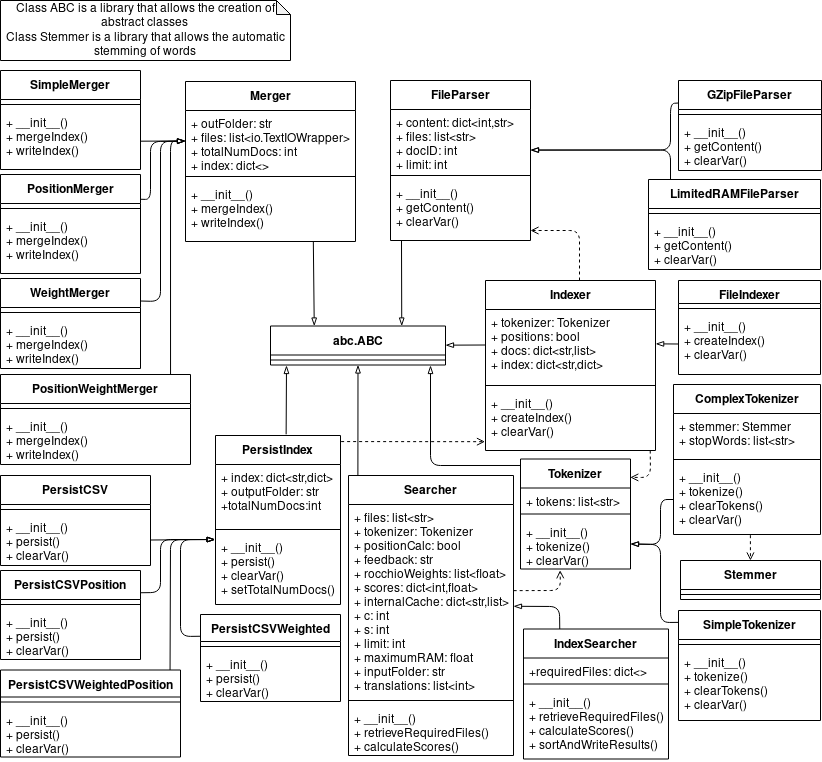
\includegraphics[width=\linewidth]{ClassDiagram_assign3.png}
\caption{Program's class diagram.}
\label{fig:classdiagram}
\end{figure}

\newpage
\section{Evaluation and Results Discussion}

In order to evaluate the quality of our solutions, with and without relevance 
feedback, we calculate an assortment of performance metrics.
The chosen metrics were: Precision, Recall, F-Measure, Mean Precision at rank 10, 
Mean Precision, Normalized Discounted Cumulative Gain, and all the averages in 
between the queries performed for all the previous metrics.
The implementation of the calculations was done in \texttt{QueryAnalyzer.py}.
Time related metrics were also considered, such as: Query Throughput and Median 
Query Latency, but for these we chose to use an auxiliary linux command line 
program called \texttt{time} which is able to summarize the system resources 
used in a program's execution.

In this chapter we explain the metrics used to evaluate the implemented ranked
retrieval, present the results of our evaluation and our discussion regarding 
them and attempt to understand what exactly are the solutions limitations.

\subsection{Evaluation Metrics}

Precision and recall are one of the most used metrics in information retrieval.
The first is characterized by dividing the correct retrieved documents by the 
totality of retrieved documents. 
This metric provides the percentage of the retrieved documents that are really 
relevant for the user.
The second consists of dividing the correct retrieved documents by the totality 
of ideal correct documents. 
The result is the percentage of correct documents the system can present.

F-Measure (or F-Score) is a metric many times used to represent the system 
performance with only one value. 
This is accomplish by the combination of the two previous metrics, performing 
the harmonic mean between the two metrics through the following equation:

\begin{equation}
  Fs = \frac{2 \times P \times R}{P + R}
\end{equation}

Mean Precision is a variation of the Precision metric. 
Its formula is similar, the difference is that in this case the precision 
is calculated in the various ranks, i.e. it is calculated for every newly 
retrieved document and then the average of all the intermediate precisions 
is achieved, resulting in the mean of the precisions of the query result
(hence the name).
Mean Precision at rank 10 is described as the Mean Precision calculated just 
until rank 10 (unitl the $10^{th}$ value).

Normalized Discounted Cumulative Gain is a more complex metric that uses a graded 
relevance scale of documents to evaluate usefulness/gain of the returned results. 
The core idea with this metric is that relevant documents that are lower in the 
list should be penalized, since the important documents should be the first 
results provided. 
This is accomplished by the formula:

\begin{equation}
  DCG = \sum_{i=1}^{p} \frac{rel_{i}}{\log_{2}(i+1)}
\end{equation}

The normalization is then achieved by dividing this value by the ideal one, i.e.
having the relevances in order, the first documents considered the most relevant 
and so on.

Query Throughput is a time related metric that indicates how many queries can be 
processed in one second. 
It's obvious that it's ideal that the information gathering and ordering should 
take the least amount of time possible, so the higher the query throughput the better.

Finally, the Median Query Latency, as the name suggests, is the average time it
takes to process a query. 
Following the same logical line of thought of the previous metric, the lower 
this number is the better, since it means that more queries can be processed in 
less time.

\subsection{Results}\label{results}

The tests phase of the project was conducted with the help of \texttt{QueryIndex}
to execute the ranked retrievals and \texttt{QueryAnalyzer} to evaluate the results.
They considered the original dataset indexed with the updates mentioned in chapter 
1 and all 50 given queries.

\texttt{QueryIndex.py} works as the script that creates an instance of the 
\texttt{IndexSearcher} and, for each query, tells it to retrieve the best results.
The command works as follows:

\begingroup
\addtolength\leftmargini{-0.4in}
\addtolength\baselineskip{-0.05in}
\begin{quote}
\begin{verbatim}
$ python3 QueryIndex.py [-h] [-p] [-o outputFile] [-t tokenizer] 
  [-r limitRAM] [-f feedback] [-n n] [-k k] [-l limit] queryFile 
  indexFolder [a b g]
\end{verbatim}
\end{quote}
\endgroup

Here, \texttt{-h} is the option that presents the manual for the command usage.
Option \texttt{-p}, if present, tell the program that the index has the positions
of each term in each document along with the weights.
Option \texttt{-o} allows the definition of the output folder's name where the
results will be stored.
Option \texttt{-t} makes possible for the user to choose the type of tokenizer
to be used, and the alternatives are: 'simple' for the use of the 
\texttt{SimpleTokenizer} class, and 'complex' for the \texttt{ComplexTokenizer} class.
The chosen tokenizer must be the same used when indexing the text corpus.
Option \texttt{-r} allows the user to define the maximum amount of memory that can
be used by the process running the program.
Option \texttt{-f} makes possible for the user to choose a form of relevance 
feedback, so that there is a greater assurance that the returned documents are
actually relevant to the query.
The alternatives are: 'pseudo' and 'user'.
Options \texttt{-n}, \texttt{-k} and \texttt{-l} allow the definition of the 
number of retrieved documents considered for the Rocchio algorithm (applyed in
the relevance feedback), the size of the champions list and the number of scores
to return (to store in the output files).
The previous arguments are all optional and the actual values for these arguments
must appear right after the respective options.
\texttt{QueryFile} and \texttt{indexFolder} are the only obligatory parameters,
as they tell the program where are the queries and the index files.
\texttt{A}, \texttt{b} and \texttt{g} are optional parameters that must be defined
if the relevance feedback is activated (if \texttt{-f} and \texttt{-n} are also
defined), as they correspond to the Rocchio algorithm's parameters alpha, beta
and gamma.

We executed \texttt{QueryIndex.py} for different combinations of parameters to
ensure its correct functioning and to search for the configuration with highest 
performances.
It was initially tested with indexes with positions and both types of tokenizers, 
although the remaining tests were all using only weights to reduce execution times
and only the complex tokenizer to remove noise and increase precision.
Then we tested the program with and without champions list (although this was
not done through the command's parameters) and for champions lists of different sizes.
Following we also varied the number of documents the program returned.
And finally we tested the program with relevance feedback, with both pseudo and
simulated user feedbacks, and with different Rocchio parameters values.

The presence of the champions list seemed to have no relevant impact on the 
overall performance, with the tests at the time rounding the 19\% of precision
(with a champions list of size 10 000).
This feature was important for the execution times, as it reduced the search 
space of the program for each query without loosing valuable information.
What we later understood was that, if its size was reduced, the lost of useful
information and relevant documents started to have a big inpact on the performance,
as for a list of size 1000 the precision dropped to about 16\%.

With the champions list at size 10 000, we tried to reduce the number of results
returned from 100 to 50, 20 and 10. 
The later reached a precision of 26\%, which was good news to us.

Although pseudo feedback was also part of our tests, we new \textit{a priori} 
that this would not influence the results at all, since it assumed that the first
results the program already considered more relevant were in fact relevant and 
increased their final scores.
User feedback, on the other hand, proved to have great value when tested.
.............................







\subsection{Discussion}\label{discussion}

Lorem ipsum ...

+ champions list = + precision
user feedback = + precision
+ results returned = - precision

low recall is normal since we return X and X can be a very small group compared to the entire universe of documents

\subsection{Implementation Limitations}

Lorem ipsum ...

\section{Conclusions}

After completing the assignment, we drew a few conclusions regarding our
solutions and the whole concept of ...........

The biggest challenge we faced was ......... rocchio, memory

From this assignment, we take ........

The overall perspective of our performance regarding the project is ..........

\begin{thebibliography}{9}
  \bibliographystyle{Science}

  \bibitem{assign3}
    S. Matos,
    \textit{IR: Assignment 3},
    University of Aveiro,
    2019/20.
  
\end{thebibliography}

\clearpage

\end{document}




















